\documentclass[main.tex]{subfiles}

\begin{document}

\addtolength{\tabcolsep}{-2pt}

\section{Parallelism}
This chapter covers the basics of parallelism and how to examine the performance of a parallel program. Recall that when we talk about parallelism, we mean the use of additional computational resources to solve a problem faster. The exercises in this chapter will usually ask you to implement a parallel algorithm to solve a certain problem, to recognize the issue of a given implementation and to analyze the performance of an implementation. 
\subsection{Performance}
\subsubsection{Speedup}
Before we begin to have a look at different ways of measuring performance, we first need to introduce some terminology. To that end, let $P$ denote the number of processors available during the execution of a program.
\begin{definition} 
$\mathbf{T_P}$ is the time it takes the program to execute on $P$ processors.
\begin{remark}
$T_\infty$ denotes the execution time when we have as many processors at our disposal as is required to get the best-possible execution time.
\end{remark}
\end{definition}
We will usually use $T_1$ to talk about the \textit{sequential} and $T_\infty$ to talk about the \textit{minimum} execution time of a program. When talking about performance in general, we will use $T_P$.
\begin{definition}
The \textbf{speedup} of a program is
\begin{equation*}
    S_P := \frac{T_1}{T_P}
\end{equation*}
\end{definition}
The speedup is essentially the ratio of the sequential execution time to the execution time given $P$ processors.\\
Naively, we might expect the speedup of our program to always be $S_P = P$, i.e. $T_P = T_1 / P$. However, reality is often disappointing. In reality, additional overheads caused by inter-thread dependencies, creating threads and communicating between them and memory-hierarchy issues can greatly limit the speedup we gain from adding more processors.

%==============================================================================================================================

\subsubsection{Amdahl's Law}
We noted in the previous section that the speedup of a given parallel program can be greatly decreased due to overhead caused by several issues introduced by parallelizing the program. In fact, any sequential parts of a program can drastically impact the maximum achievable speedup. We will derive Amdahl's law here to see why this is the case.\\
\\
Let $W_{ser}$ denote the time spent doing non-parallelizable, serial work and $W_{par}$ denote the time spent doing parallelizable work.\\
We then write:
\begin{equation*}
    T_1 = W_{ser} + W_{par}
\end{equation*}
It's easy to see that $T_{ser}$ remains constant as we increase the number of processors. Therefore, given $P$ processors, we obtain the following lower bound on $T_P$:
\begin{equation*}
    T_P \geq W_{ser} + \frac{W_{par}}{P}
\end{equation*}
Recall the definition of speedup. Plugging in the relations derived above, we get:
\begin{equation*}
    S_P = \frac{T_1}{T_P} \leq \frac{W_{ser} + W_{par}}{W_{ser} + \frac{W_{par}}{P}}
\end{equation*}
Let $\mathbf{f}$ denote the non-parallelizable, serial fraction of the total work. We then obtain the following equalities:
\begin{gather*}
    W_{ser} = \mathbf{f}*T_1 \\
    W_{par} = (1-\mathbf{f})*T_1
\end{gather*}
This gives us the more common form of Amdahl's Law:
\begin{theorem} 
    Let $\mathbf{f}$ denote the non-parallelizable, serial fraction of the total work done in a program and $P$ the number of processors at our disposal. Then, the following inequality holds:
    \begin{equation*}
        S_P \leq \frac{1}{\mathbf{f} + \frac{1-\mathbf{f}}{P}}
    \end{equation*}
\end{theorem}
When we let $P$ go to $\infty$, we see:
\begin{equation*}
    S_\infty \leq \frac{1}{\mathbf{f}}
\end{equation*}
In order to see why this is such an important result, we can try plugging in a couple of values. Assume that 25\% of a program is non-parallelizable. This means that even with the \textit{IBM Blue Gene/P} supercomputer with its 164'000 cores, we can only achieve a speedup of at most 4. While a depressing result at first sight, this makes perfect sense when we consider the fact that these 25\% are completely fixed, in the sense that the execution time can't possibly be reduced past this point.\\[0.3cm]
The conclusion we can draw from this result is that it's worth investing some more time into reducing the sequential fraction of our program, e.g. by reducing the overhead of communicating between threads or by reducing the granularity of locks in our code as much as possible.

%==============================================================================================================================

\subsubsection{Gustafson's Law}
Amdahl's law considered a fixed workload and provides us with an upper bound on the speedup achievable when increasing the number of processors at our disposal. As the obtained result is rather depressing, we seek to find something slightly more optimistic. This leads us to an approach where we increase the problem size as we improve the resources at our disposal. In other words, we consider the time interval to be fixed and look at the problem size.\\
Let $W$ denote the work done in a fixed time interval. We get
\begin{equation*}
    W = \mathbf{f} * W + (1 - \mathbf{f}) * W
\end{equation*}
As we increase the number of processors at our disposal, we can only speed up the parallel fraction of our program. The serial fraction remains the same. Letting $W_P$ be the work done with $P$ processors at our disposal, we get
\begin{equation*}
    W_P = \mathbf{f} * W + P * (1 - \mathbf{f}) * W
\end{equation*}
We can now follow \textit{Gustafson's law}.
\begin{theorem}
    Let $\mathbf{f}$ denote the non-parallelizable, serial fraction of the total work done in the program and P the number of processors at our disposal. Then, we get
    \begin{align*}
        S_P &= \mathbf{f} + P(1-f)\\
            &= P - \mathbf{f}(P-1)
    \end{align*}
\end{theorem}
If we again consider a program where 25\% is non-parallelizable, we get a speedup of 4 when we increase the number of processors to 5.

\pagebreak
%==============================================================================================================================
%==============================================================================================================================

\subsection{Divide \& Conquer}
In divide \& conquer we split a problem into smaller subproblems, solve the task recursively for each of these and combine the results such that we obtain the final result for the entire problem. To see how this approach works, let's construct a small example:
\begin{example}
    Through some weird twist of faith, we're given a list of the number of clocks each Swiss citizen posseses and are tasked with finding the maximum among all of these. For the sake of simplicity, suppose this list only has eight entries. 
    \begin{center}
        15\quad 7\quad 9\quad 8\quad 4\quad 22\quad 42\quad 13
    \end{center}
    The first step of a divide \& conquer algorithm is to divide the problem into smaller subproblems.
    \begin{center}
        \hspace*{\fill} 15\quad 7\quad 9\quad 8 \hspace*{\fill} 4\quad 22\quad 42\quad 13 \hspace*{\fill}
    \end{center}
    We then continue on like this until we reach a base case. Note that we break the list into single numbers and not into pairs of numbers. The reason for this is that the list might have an odd length, which of course couldn't be broken into pairs of numbers.
    \begin{center}
        \hspace*{\fill} 15 \hspace*{\fill} 7 \hspace*{\fill} 9 \hspace*{\fill} 8 \hspace*{\fill} 4 \hspace*{\fill} 22 \hspace*{\fill} 42 \hspace*{\fill} 13 \hspace*{\fill}
    \end{center}
    Then we begin to find the maximum, 2 numbers at a time.
    \begin{center}
        \hspace*{\fill} 15 \hspace*{\fill}  9 \hspace*{\fill} 22 \hspace*{\fill} 42 \hspace*{\fill}
    \end{center}
    We continue on like this until only one number remains.
    \begin{center}
        42
    \end{center}
    We've thus come to the conclusion that the largest number of clocks possessed by a single person in Switzerland is 42.
\end{example}
This algorithm consisted of three steps. First, we broke the list into two smaller lists. This is known as the ''divide'' step. Then, we solved the task for each of these sublists. This is known as the ''conquer'' step. Finally, we combined the results of the subproblems by taking the maximum of the two returned maxima.\\[0.3cm]
While divide \& conquer algorithms seem very natural to parallelize, we currently have no easy way of determining the efficiency of these algorithms in a parallel setting and it's quite tedious to implement using regular Java threads. We will therefore first introduce a way of visualizing the performance of a divide \& conquer algorithm and will then look at two different libraries to see how we can easily implement this.

%==============================================================================================================================

\subsubsection{Task Graphs}
We will describe a program execution as a directed acyclic graph where:
\begin{itemize}
    \item Nodes are pieces of work the program performs. Each node will have a constant execution time per task. In most cases we will interpret the execution time per node as 1.
    \item Edges represent that the source node must complete before the target node begins, i.e. there is a data dependency along the edge.
\end{itemize}
We will now connect this visual representation of the execution of a program with the terminology introduced in the previous section by introducing two more terms:
\begin{itemize}
    \item \textbf{Work} is the sum of the time cost of all nodes in the graph, i.e. $T_1$.
    \item  \textbf{Span} is the sum of the time cost of all nodes along the critical, i.e. longest, path in the graph. The span determines the best possible execution time we can achieve by introducing more processors, i.e. $T_\infty$.
\end{itemize}
\begin{example}
    Let's return to our example from the previous section where we try to find the largest number of clocks currently owned by a Swiss citizen. Assume that splitting a list into two sublists can be done in 3 ''time units'', finding the maximum can be done in 2 units and appending two lists can be done in 4 units.\\[0.3cm]
    The task graph will then look like this:
    \begin{center}
        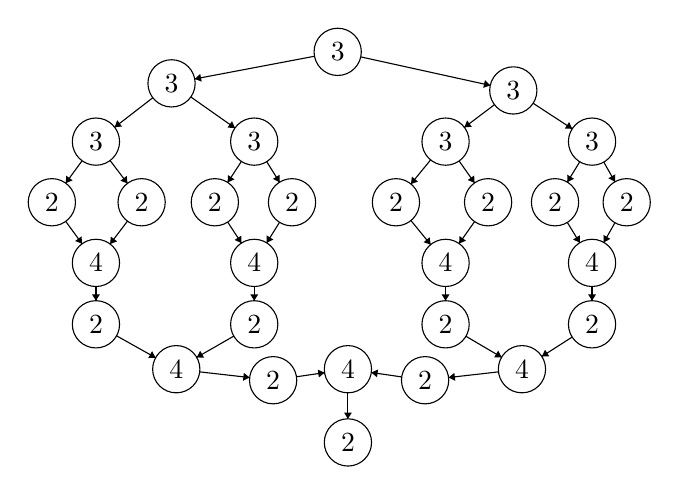
\begin{tikzpicture}[scale=0.1]
            \tikzstyle{every node}+=[inner sep=0pt]
            \draw [black] (40.1,-5.4) circle (3);
            \draw (40.1,-5.4) node {$3$};
            \draw [black] (19,-9.4) circle (3);
            \draw (19,-9.4) node {$3$};
            \draw [black] (62.4,-10.3) circle (3);
            \draw (62.4,-10.3) node {$3$};
            \draw [black] (9.4,-16.8) circle (3);
            \draw (9.4,-16.8) node {$3$};
            \draw [black] (29.5,-16.8) circle (3);
            \draw (29.5,-16.8) node {$3$};
            \draw [black] (53.8,-16.8) circle (3);
            \draw (53.8,-16.8) node {$3$};
            \draw [black] (72.4,-16.8) circle (3);
            \draw (72.4,-16.8) node {$3$};
            \draw [black] (3.8,-24.5) circle (3);
            \draw (3.8,-24.5) node {$2$};
            \draw [black] (15.2,-24.5) circle (3);
            \draw (15.2,-24.5) node {$2$};
            \draw [black] (24.5,-24.5) circle (3);
            \draw (24.5,-24.5) node {$2$};
            \draw [black] (34.3,-24.5) circle (3);
            \draw (34.3,-24.5) node {$2$};
            \draw [black] (47.5,-24.5) circle (3);
            \draw (47.5,-24.5) node {$2$};
            \draw [black] (59.2,-24.5) circle (3);
            \draw (59.2,-24.5) node {$2$};
            \draw [black] (67.7,-24.5) circle (3);
            \draw (67.7,-24.5) node {$2$};
            \draw [black] (76.8,-24.5) circle (3);
            \draw (76.8,-24.5) node {$2$};
            \draw [black] (9.4,-32.2) circle (3);
            \draw (9.4,-32.2) node {$4$};
            \draw [black] (29.5,-32.2) circle (3);
            \draw (29.5,-32.2) node {$4$};
            \draw [black] (53.8,-32.2) circle (3);
            \draw (53.8,-32.2) node {$4$};
            \draw [black] (72.4,-32.2) circle (3);
            \draw (72.4,-32.2) node {$4$};
            \draw [black] (9.4,-40) circle (3);
            \draw (9.4,-40) node {$2$};
            \draw [black] (29.5,-40) circle (3);
            \draw (29.5,-40) node {$2$};
            \draw [black] (53.8,-40) circle (3);
            \draw (53.8,-40) node {$2$};
            \draw [black] (72.4,-40) circle (3);
            \draw (72.4,-40) node {$2$};
            \draw [black] (19.6,-45.7) circle (3);
            \draw (19.6,-45.7) node {$4$};
            \draw [black] (63.5,-45.7) circle (3);
            \draw (63.5,-45.7) node {$4$};
            \draw [black] (31.9,-47.1) circle (3);
            \draw (31.9,-47.1) node {$2$};
            \draw [black] (51.2,-47.1) circle (3);
            \draw (51.2,-47.1) node {$2$};
            \draw [black] (41.4,-45.7) circle (3);
            \draw (41.4,-45.7) node {$4$};
            \draw [black] (41.4,-55) circle (3);
            \draw (41.4,-55) node {$2$};
            \draw [black] (43.03,-6.04) -- (59.47,-9.66);
            \fill [black] (59.47,-9.66) -- (58.8,-9) -- (58.58,-9.97);
            \draw [black] (37.15,-5.96) -- (21.95,-8.84);
            \fill [black] (21.95,-8.84) -- (22.83,-9.18) -- (22.64,-8.2);
            \draw [black] (16.62,-11.23) -- (11.78,-14.97);
            \fill [black] (11.78,-14.97) -- (12.71,-14.88) -- (12.1,-14.08);
            \draw [black] (21.45,-11.13) -- (27.05,-15.07);
            \fill [black] (27.05,-15.07) -- (26.68,-14.2) -- (26.11,-15.02);
            \draw [black] (60.01,-12.11) -- (56.19,-14.99);
            \fill [black] (56.19,-14.99) -- (57.13,-14.91) -- (56.53,-14.11);
            \draw [black] (64.92,-11.93) -- (69.88,-15.17);
            \fill [black] (69.88,-15.17) -- (69.49,-14.31) -- (68.94,-15.15);
            \draw [black] (7.64,-19.23) -- (5.56,-22.07);
            \fill [black] (5.56,-22.07) -- (6.44,-21.72) -- (5.63,-21.13);
            \draw [black] (11.2,-19.2) -- (13.4,-22.1);
            \fill [black] (13.4,-22.1) -- (13.31,-21.16) -- (12.51,-21.77);
            \draw [black] (27.87,-19.32) -- (26.13,-21.98);
            \fill [black] (26.13,-21.98) -- (26.99,-21.59) -- (26.15,-21.04);
            \draw [black] (31.09,-19.35) -- (32.71,-21.95);
            \fill [black] (32.71,-21.95) -- (32.71,-21.01) -- (31.87,-21.54);
            \draw [black] (51.9,-19.12) -- (49.4,-22.18);
            \fill [black] (49.4,-22.18) -- (50.29,-21.88) -- (49.52,-21.24);
            \draw [black] (55.52,-19.26) -- (57.48,-22.04);
            \fill [black] (57.48,-22.04) -- (57.43,-21.1) -- (56.61,-21.68);
            \draw [black] (70.84,-19.36) -- (69.26,-21.94);
            \fill [black] (69.26,-21.94) -- (70.11,-21.52) -- (69.25,-21);
            \draw [black] (73.89,-19.4) -- (75.31,-21.9);
            \fill [black] (75.31,-21.9) -- (75.35,-20.95) -- (74.48,-21.45);
            \draw [black] (5.56,-26.93) -- (7.64,-29.77);
            \fill [black] (7.64,-29.77) -- (7.57,-28.83) -- (6.76,-29.42);
            \draw [black] (13.4,-26.9) -- (11.2,-29.8);
            \fill [black] (11.2,-29.8) -- (12.09,-29.47) -- (11.29,-28.86);
            \draw [black] (26.13,-27.02) -- (27.87,-29.68);
            \fill [black] (27.87,-29.68) -- (27.85,-28.74) -- (27.01,-29.29);
            \draw [black] (32.71,-27.05) -- (31.09,-29.65);
            \fill [black] (31.09,-29.65) -- (31.93,-29.24) -- (31.09,-28.71);
            \draw [black] (49.4,-26.82) -- (51.9,-29.88);
            \fill [black] (51.9,-29.88) -- (51.78,-28.94) -- (51.01,-29.58);
            \draw [black] (57.48,-26.96) -- (55.52,-29.74);
            \fill [black] (55.52,-29.74) -- (56.39,-29.38) -- (55.57,-28.8);
            \draw [black] (69.26,-27.06) -- (70.84,-29.64);
            \fill [black] (70.84,-29.64) -- (70.85,-28.7) -- (69.99,-29.22);
            \draw [black] (75.31,-27.1) -- (73.89,-29.6);
            \fill [black] (73.89,-29.6) -- (74.72,-29.15) -- (73.85,-28.65);
            \draw [black] (9.4,-35.2) -- (9.4,-37);
            \fill [black] (9.4,-37) -- (9.9,-36.2) -- (8.9,-36.2);
            \draw [black] (29.5,-35.2) -- (29.5,-37);
            \fill [black] (29.5,-37) -- (30,-36.2) -- (29,-36.2);
            \draw [black] (53.8,-35.2) -- (53.8,-37);
            \fill [black] (53.8,-37) -- (54.3,-36.2) -- (53.3,-36.2);
            \draw [black] (72.4,-35.2) -- (72.4,-37);
            \fill [black] (72.4,-37) -- (72.9,-36.2) -- (71.9,-36.2);
            \draw [black] (56.39,-41.52) -- (60.91,-44.18);
            \fill [black] (60.91,-44.18) -- (60.48,-43.34) -- (59.97,-44.21);
            \draw [black] (69.87,-41.62) -- (66.03,-44.08);
            \fill [black] (66.03,-44.08) -- (66.97,-44.07) -- (66.43,-43.23);
            \draw [black] (12.02,-41.46) -- (16.98,-44.24);
            \fill [black] (16.98,-44.24) -- (16.53,-43.41) -- (16.04,-44.28);
            \draw [black] (26.9,-41.5) -- (22.2,-44.2);
            \fill [black] (22.2,-44.2) -- (23.14,-44.24) -- (22.64,-43.37);
            \draw [black] (60.52,-46.04) -- (54.18,-46.76);
            \fill [black] (54.18,-46.76) -- (55.03,-47.17) -- (54.92,-46.17);
            \draw [black] (22.58,-46.04) -- (28.92,-46.76);
            \fill [black] (28.92,-46.76) -- (28.18,-46.17) -- (28.07,-47.17);
            \draw [black] (34.87,-46.66) -- (38.43,-46.14);
            \fill [black] (38.43,-46.14) -- (37.57,-45.76) -- (37.71,-46.75);
            \draw [black] (48.23,-46.68) -- (44.37,-46.12);
            \fill [black] (44.37,-46.12) -- (45.09,-46.73) -- (45.23,-45.74);
            \draw [black] (41.4,-48.7) -- (41.4,-52);
            \fill [black] (41.4,-52) -- (41.9,-51.2) -- (40.9,-51.2);
        \end{tikzpicture}
    \end{center}
    Let's say we now wish to compute the maximum achievable speedup we can gain by parallelizing this algorithm, i.e. $S_\infty$. We know that the formula for speedup is
    \begin{equation*}
        S_P = \frac{T_1}{T_P}
    \end{equation*}
    $T_1$ is defined as the sum of the time cost all nodes in the graph, which in this case would be 79.  We can compute $T_\infty$ as the sum of the time cost of all nodes along the critical path, which we see is 29. As a final result, we thus obtain
    \begin{equation*}
        S_\infty = \frac{79}{29} \approx 2.72
    \end{equation*}
    We recognize from the width of the graph that we can issue at most 8 operations in parallel. This means that we achieve $T_\infty$ with 8 processors, i.e. $S_8 = S_\infty$
\end{example}

%==============================================================================================================================

\subsubsection{Executor Service}
Instead of managing the threads ourselves we can use a library which manages a threadpool to which we can submit tasks. A task is either:
\begin{itemize}
    \item A \texttt{Runnable} object, which implements a method \texttt{void run()} and doesn't return a result
    \item or a \texttt{Callable$<$T$>$} object, which implements a method \texttt{T call()} and returns a result of type \texttt{T}.
\end{itemize}
Upon submitting a task a \texttt{Future$<$T$>$} is created, which contains the result of the submitted task. Implementing a divide \& conquer algorithm now looks a lot more straightforward.

\newpage

\begin{example}
    We wish to submit tasks to the \texttt{ExecutorService} such that we can obtain some sort of result from the task's execution. We therefore need to implement a \texttt{Callable} task (i). We've additionally provided the code for creating an \texttt{ExecutorService} and submitting the topmost task (ii). Try running it locally and see what happens. 
    \begin{figure}[H]
        \centering
        \begin{subfigure}{.5\textwidth}
            \centering
            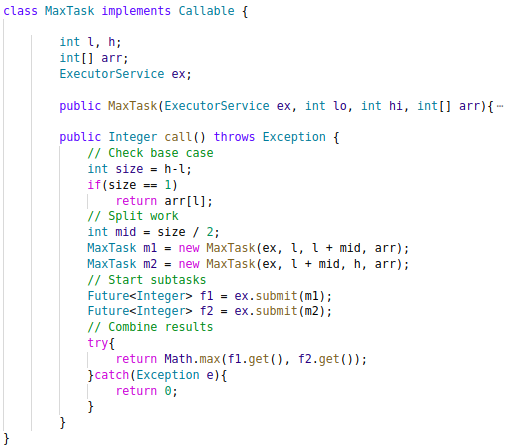
\includegraphics[scale=0.45]{ExecutorService.png}
            \caption{implementation of \texttt{Callable} task}
        \end{subfigure}%
        \begin{subfigure}{.5\textwidth}
            \centering
            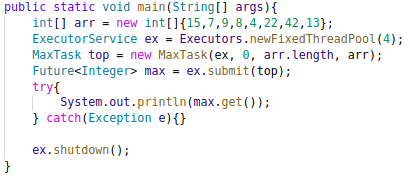
\includegraphics[scale=0.45]{ExecutorServiceMain.png}
            \caption{implementation of \texttt{main} method}
        \end{subfigure}
    \end{figure}
    \noindent You should see that the program never terminates. The reason for this is that the \texttt{ExecutorService} limits the number of threads that can be spawned. Once all threads are occupied by tasks waiting for the result of spawned subtasks, execution is therefore halted. No threads are available to run the subtasks on, i.e. the subtasks will wait indefinitely.
\end{example}
With the \texttt{ExecutorService} the limited thread pool size caused the program to run forever, as all currently active threads were occupied by tasks waiting for the spawned subtasks to return. While there are possible approaches that could alleviate this problem, e.g. seperating the work partitioning from solving the sub-tasks, they are all non-trivial to implement and are therefore not well suited for use in practice.

%==============================================================================================================================

\subsubsection{Fork/Join Framework}
We continue our search for a library well-suited to implementing divide \& conquer algorithms. The \texttt{java.util.concurrent} package includes classes designed exactly for this type of fork-join parallelism.\\
Compared to Java threads, the usage of these classes is exactly the same, but with some different names and interfaces. First, we'll introduce the required terminology. Second, we'll have a look at the generic recipe for implementing fork-join parallelism.\\
\\
We use the library as follows:
\begin{itemize}
    \item Instead of extending \texttt{Thread}, we extend \texttt{RecursiveTask$<$T$>$} (with return value) or \texttt{RecursiveAction} (without return value)
    \item Instead of overriding \texttt{run}, we override \texttt{compute}
    \item Instead of calling \texttt{start}, we call \texttt{fork}
    \item Instead of a topmost call to \texttt{run}, we create a \texttt{ForkJoinPool} and call \texttt{invoke}
\end{itemize}
Also, note that in the case of \texttt{RecursiveTask$<$T$>$}, \texttt{join} now returns a result.\\
\begin{example}
    We again return to our previous example of trying to find the largest number of clocks currently owned by any Swiss citizen. We'd again like our tasks to return a result. We therefore need to implement a \texttt{RecursiveTask<T>} (i). We've additionally provided the code for creating a \texttt{ForkJoinPool} and submitting the topmost task (ii). Try running it locally and see if it works this time around. \\
    \\
    \begin{figure}[H]
        \centering
        \begin{subfigure}{.5\textwidth}
            \centering
            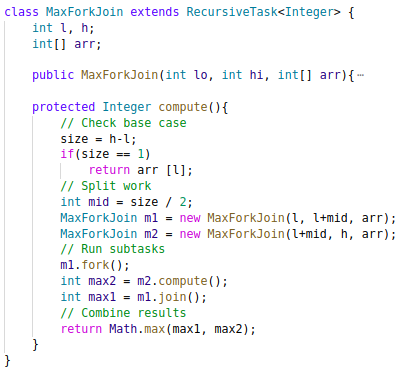
\includegraphics[scale=0.45]{GenericForkJoin.png}
            \caption{Implemention of \texttt{RecursiveTask}}
        \end{subfigure}%
        \begin{subfigure}{.5\textwidth}
            \centering
            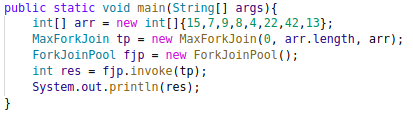
\includegraphics[scale=0.45]{ForkJoinMain.png}
            \caption{Implementation of \texttt{main} method}
        \end{subfigure}
    \end{figure}
    \noindent Several things should be noted in this example. First, changing anything about the order in which the subtasks were called will result in a sequential execution (try it!). Second, similar to how we did it for regular threads, we call \texttt{compute()} instead of submitting another task using \texttt{fork()}.\\
    Both in the case of the \texttt{ForkJoin}-framework and of \texttt{ExecutorService}, one should pay extra attention as to how to split the array such that all indices are covered exactly once. In this example and example 2.3, note the way the middle index was computed and think about what indices the \texttt{h} and \texttt{l} variables represented exactly.
\end{example}
\pagebreak
%==============================================================================================================================
%==============================================================================================================================

\subsection{Pipelining}
There are three approaches to applying parallelism to improve sequential processor performance. The first is vectorization, where we essentially apply operations N-at-a-time, as opposed to the standard one-at-a-time approach. The second is instruction level parallelism, where we ask ourselves which instructions are independent of each other and can therefore be executed in parallel and/or reordered. This is where keywords such as superscalar CPUs and out-of-order execution come into play. The third and most important approach that we will consider is pipelining. \\[3mm]
Pipelining is a technique where multiple independent instructions are overlapped in execution through the use of multiple execution units, provided they are available for use.
\begin{definition}
    \textbf{Throughput} is the number of instructions that exit the pipeline per a given time unit. Throughput can be calculated as follows:
    \begin{equation*}
        Throughput \approx \frac{1}{max(computationtime(stages))}
    \end{equation*}
\end{definition}
Note that we usually consider throughput when the pipeline is fully utilized, i.e. ignoring lead-in and lead-out time.
\begin{definition}
    \textbf{Latency} is the time to perform a single computation, including wait time resulting from resource dependencies.
\end{definition}
When designing a pipeline, it's of course always our aim to increase throughput and decrease latency as much as possible. However, the two goals are often conflicting.
\begin{definition}
    A pipeline is \textbf{balanced} if the latency remains constant over time.
\end{definition}
\begin{example}
    We return to the good old washing cycle pipeline, only with a little twist this time around. The stages of the washing cycle consist of first using the washing machine, then the dryer, folding the washing, and finally putting it away in the closet. The washing machine is quite a cheap brand and takes 15 seconds per washing (as opposed to the usual 5 seconds). The dryer takes 10 seconds, folding the washing 5 seconds, and putting it away in the closet another 5 seconds.\\[3mm]
    \begin{tabular}{l | *{19}{c}}
        Time (s) & 0 & 5 & 10 & 15 & 20 & 25 & 30 & 35 & 40 & 45 & 50 & 55 & 60 & 65 & 70 & 75 & 80 & 85 & 90 \\
        \hline
        Load 1 & w & w & w & d & d & f & c\\
        Load 2 &   &   &   & w & w & w & d & d & f & c\\
        Load 3 &   &   &   &   &   &   & w & w & w & d & d & f & c \\
        Load 4 &   &   &   &   &   &   &   &   &   & w & w & w & d & d & f & c \\
        Load 5 &   &   &   &   &   &   &   &   &   &   &   &   & w & w & w & d & d & f & c
    \end{tabular} \\[3mm]
    Looking at the definitions above, we find that the latency is 30 seconds and the throughput is 1 load per 15 seconds. In order to improve our throughput, we buy a new washing machine and give away the old one to charity. The new execution time for the washing stage is 5 seconds. \\[3mm]
    \begin{tabular}{l | *{19}{c}}
        Time (s) & 0 & 5 & 10 & 15 & 20 & 25 & 30 & 35 & 40 & 45 & 50 & 55 & 60 & 65 & 70 & 75 & 80 & 85 & 90 \\
        \hline
        Load 1 & w & d & d & f & c\\
        Load 2 &   & w & - & d & d & f & c\\
        Load 3 &   &   & w & - & - & d & d & f & c \\
        Load 4 &   &   &   & w & - & - & - & d & d & f & c \\
        Load 5 &   &   &   &   & w & - & - & - & - & d & d & f & c
    \end{tabular} \\[3mm]
    We see that our new throughput is 1 load per 10 seconds. Latency, however, seems to be increasing, i.e. the pipeline is now unbalanced. 
\end{example}
\noindent This example illustrated one important problem that can occur in pipelines. Despite achieving a high throughput, the latency increased indefinitely.
Over the years it has become evident that improving sequential processor performance with methods such as these is not enough. This has led to the development of parallel architectures such as multicore processors and processors implementing simultaneous multithreading as we know them today.

\pagebreak
%==============================================================================================================================
%==============================================================================================================================

\subsection{Exercises}

\begin{ExerciseList}
    \Exercise[title={Amdahl's Law, Gustafson's Law, Performance},label=AGL].
        \Question Suppose a computer program has a method \textbf{M} that cannot be parallelized, and that this method accounts for 40\% of the program’s execution time. What is the limit for the overall speedup that can be achieved by running the program on an n-processor multiprocessor machine according to \textbf{Amdahl's Law}?
        \Question The analysis of a program has shown a speedup of 5 when running on 15 cores. What is the serial fraction according to \textbf{Amdahl's Law} (assuming best possible speedup)?
        \Question The analysis of a program has shown a speedup of 5 when running on 15 cores. What is the serial fraction according to \textbf{Gustafson's Law}?
    \Answer[ref={AGL}].
        \Question We see that the program has a serial fraction of 40\%. Therefore, we set $\mathbf{f} = 0.4$ and insert this into the formula specified by Amdahl's Law:
            \begin{equation*}
                S_P \leq \frac{1}{\mathbf{f} + \frac{1-\mathbf{f}}{P}} = \frac{1}{0.4 + \frac{0.6}{P}} \xrightarrow{P \rightarrow \infty} \frac{1}{0.4} = 2.5
            \end{equation*}
        \Question Assuming best possible speedup, Amdahl's Law tells us the following holds true
            \begin{gather*}
                S_P = 5 = \frac{1}{\mathbf{f}+\frac{1-\mathbf{f}}{P}} = \frac{1}{\mathbf{f}+\frac{1-\mathbf{f}}{15}} \\
                \Longleftrightarrow\\
                5 \mathbf{f} + \frac{1-\mathbf{f}}{3} = 5 \mathbf{f} - \frac{1}{3} \mathbf{f} + \frac{1}{3} = 1\\
                \Longleftrightarrow\\
                \mathbf{f} = \frac{1}{7}
            \end{gather*}
        \Question Gustafson's Law tells us the following holds true
            \begin{gather*}
                S_P = \mathbf{f} + P (1 - \mathbf{f})
                    = \mathbf{f} + 15 (1 - \mathbf{f})
                    = 5 \\
                \Longleftrightarrow\\
                14 \mathbf{f} = 10\\
                \Longleftrightarrow\\
                \mathbf{f} = \frac{5}{7}
            \end{gather*}
        
    \Exercise[title={Task Graph}, label=TG]. \quad The following figure shows the task graph for an algorithm. The number in each node denotes the execution time per task. What is the maximum overall achievable speedup that can be achieved by parallelism when the algorithm runs once compared to sequential execution? How many processors are required to achieve this speedup?
        \begin{figure}[h]
            \centering
            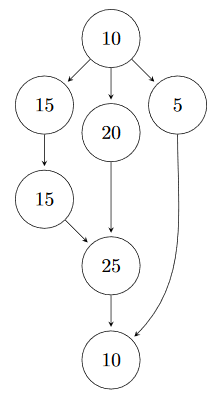
\includegraphics[scale=0.7]{TaskGraph.png}
        \end{figure}
    \Answer[ref={TG}].\quad The formula for speedup is $S_P = \frac{T_1}{T_P}$. We know that $T_1$ is the simply the sum of the execution times of all nodes, i.e. $T_1 = 100$. We also know that the best-possible execution time achievable through parallelization is limited by the length of the critical path. The critical path has length 75, i.e. $T_\infty$ = 75. Inserting these values into the formula for speedup gives us:
        \begin{equation*}
            S_\infty = \frac{T_1}{T_\infty} = \frac{100}{75} \approx 1.33
        \end{equation*}
        We find that two processors are enough to achieve this speedup.
        \pagebreak
        
    \Exercise[title={Fork/Join Framework},label=FJW].\quad Given an array of integers, your task is to find the maximum subarray sum among all possible subarrays. For example,
    \begin{center}
        \{2, -4, \textbf{1, 9, -6, 7}, -3\} $\rightarrow$ 11 (marked in \textbf{bold})
    \end{center}
    Extend the following class such that it computes the maximum subarray sum as described above.
    \begin{figure}[H]
        \centering
        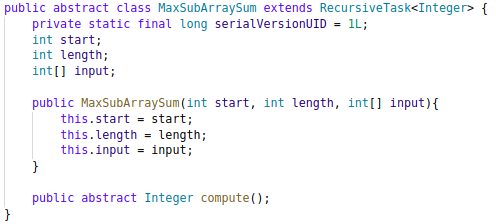
\includegraphics[scale=0.45]{MaxSubArraySum.png}
    \end{figure}
    \pagebreak
    \Answer[ref={FJW}].\quad We stick to the generic recipe for the Fork/Join framework. The difficulty with this exercise is the merging of the results of the two subtasks, as the maximum subarray sum might contain elements of both array partitions. We therefore need to additionally compute the maximum subarray sum which crosses the middle border and return the maximum of the three sums.
        \begin{figure}[H]
            \centering
            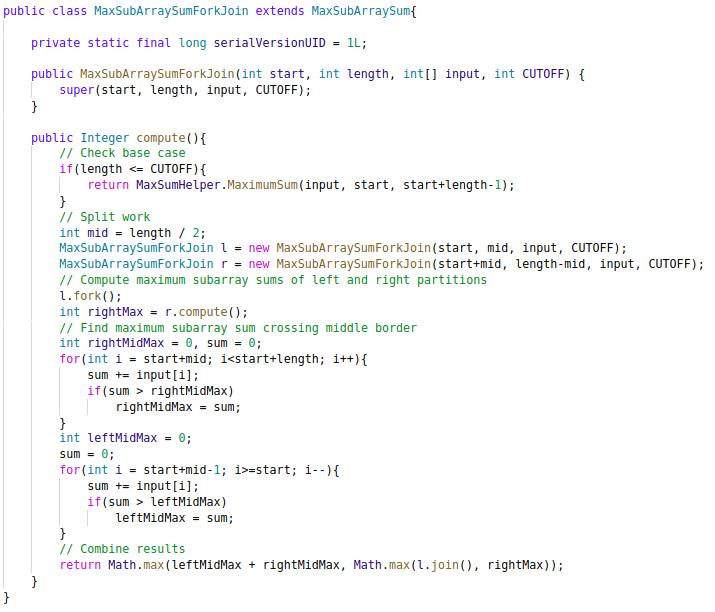
\includegraphics[scale=0.55]{MaxSubArraySumForkJoin_Sol.png}
        \end{figure}
    
    \Exercise[title={Pipelining},label=pipe].\quad Over at UZH the law students have been tasked with writing a legal essay about the philosophy of Swiss law. In order to write the essay, a student first needs to inform themselves about the subject. To do so, they must read from four different books, each of which contains information necessary to understand the next book. \\[3mm]
    Every student takes the exact same amount of time to read a book, namely:
    \begin{enumerate}[label=\arabic*)]
        \item\ Reading book A takes 80 minutes
        \item\ Reading book B takes 40 minutes
        \item\ Reading book C takes 120 minutes
        \item\ Reading book D takes 40 minutes
    \end{enumerate}
        \Question Let's assume all law students are a bit too competitive and don't return any books before they're done reading all of them. How long will it take for 4 students until all of them have started writing their essays?
        \Question The library introduces a ''one book at a time'' policy, i.e. the students have to return a book before they can start on the next one. How long will it now take for 4 students until all of them have started writing their essays? What is the throughput of this ''pipeline'' per hour? What is the latency?
        \Question Where is the problem with this system? What can the library do to solve this problem?
    \Answer[ref={pipe}].\\
        \Question In the case of a sequential execution we simply need to add the execution times of the four stages together and multiply this by the number of students.
            \begin{equation*}
                (80 + 40 + 120 + 40) * 4 = 280 * 4  = 1120 \text{ minutes}
            \end{equation*}
        \Question We assume all students immediately pick up a book as soon as it's available and they've finished reading the previous one. We can then model execution in the following way: \\[3mm]
            \begin{small}
                \begin{tabular}{l | *{19}{c}}
                    Time (s) & 0 & 40 & 80 & 120 & 160 & 200 & 240 & 280 & 320 & 360 & 400 & 440 & 480 & 520 & 560 & 600 & 640 & 680 & 720 \\
                    \hline
                    Load 1 & A & A & B & C & C & C & D\\
                    Load 2 &   &   & A & A & B & - & C & C & C & D\\
                    Load 3 &   &   &   &   & A & A & B & - & - & C & C & C & D \\
                    Load 4 &   &   &   &   &   &   & A & A & B & - & - & - & C & C & C & D \\
                    Load 5 &   &   &   &   &   &   &   &   & A & A & B & - & - & - & - & C & C & C & D
                \end{tabular} \\[3mm]
            \end{small}
            We compute the throughput the standard way, i.e. $\text{Throughput } = \frac{1}{120}$. Therefore, throughput is 1 student per 2 hours.\\[3mm]
            When looking at the diagram above we see that the waiting time before students can read book C, and therefore also the latency, increases indefinitely.
        \Question Latency increasing indefinitely is a sign that the pipeline is unbalanced. There are several solutions to this problem. First, the library could force people to keep each book for exactly 120 minutes or, slightly more efficient, to keep book A for 120 minutes and book B for 80 minutes. Alternatively, the library could buy a second copy of book C. The reader is encouraged to model the execution and convince themselves that this would alleviate the issue. A last option would be to just split book C into two copies, effectively replacing the third stage with two stages, each with an execution time of 60 minutes.\\[3mm]
            \begin{small}
                \begin{tabular}{l | *{19}{c}}
                    Time (s) & 0 & 40 & 80 & 120 & 160 & 200 & 240 & 280 & 320 & 360 & 400 & 440 & 480 & 520 & 560 & 600 & 640 & 680 & 720 \\
                    \hline
                    Load 1 & A & A & B & C & C$\|$C' & C' & D\\
                    Load 2 &   &   & A & A & B & C & C$\|$C' & C' & D\\
                    Load 3 &   &   &   &   & A & A & B & C & C$\|$C' & C' & D \\
                    Load 4 &   &   &   &   &   &   & A & A & B & C & C$\|$C' & C' & D \\
                    Load 5 &   &   &   &   &   &   &   &   & A & A & B & C & C$\|$C' & C' & D
                \end{tabular} \\[3mm]
            \end{small}
\end{ExerciseList}
\newpage
\subsection{Solutions}
\shipoutAnswer

\end{document}